%
%\documentclass[conference]{IEEEtran}
%\usepackage{times}
%
%% numbers option provides compact numerical references in the text. 
%\usepackage[numbers]{natbib}
%\usepackage{multicol}
%\usepackage[bookmarks=true]{hyperref}
%
%\usepackage{bbm}
%\usepackage{calc}
%\usepackage{url}
%\usepackage{hyperref}
%\hypersetup{
%  colorlinks =true,
%  urlcolor = black,
%  linkcolor = black
%}
%\usepackage{graphicx}
%\usepackage[cmex10]{amsmath}
%\usepackage{bm}
%\usepackage{amssymb}
%\usepackage{rotating}
%
%
%%\usepackage{xfrac}
%\usepackage{nicefrac}
%\usepackage{cite}
%\usepackage[caption=false,font=footnotesize]{subfig}
%\usepackage[usenames, dvipsnames]{color}
%\usepackage{colortbl}
%%\usepackage{caption}
%
%%\usepackage{wrapfig}
%\usepackage{overpic}
%%\usepackage{subfigure}
%%\usepackage{textcomp}
%\graphicspath{{./pictures/pdf/},{./pictures/ps/},{./pictures/png/},{./pictures/jpg/}}
%\usepackage{breqn} %for breaking equations automatically
%\usepackage[ruled]{algorithm}
%\usepackage{algpseudocode}
%%\usepackage{algorithmic}
%\usepackage{multirow}
%\usepackage{todonotes}
%
%%\newcommand{\todo}[1]{\vspace{5 mm}\par \noindent \framebox{\begin{minipage}[c]{0.98 \columnwidth} \ttfamily\flushleft \textcolor{red}{#1}\end{minipage}}\vspace{5 mm}\par}
%% uncomment this to hide all red todos
%%\renewcommand{\todo}{}
%
%%% ABBREVIATIONS
%\newcommand{\qstart}{q_{\text{start}}}
%\newcommand{\qgoal}{q_{\text{goal}}}
%\newcommand{\pstart}{p_{\text{start}}}
%\newcommand{\pgoal}{p_{\text{goal}}}
%\newcommand{\xstart}{x_{\text{start}}}
%\newcommand{\xgoal}{x_{\text{goal}}}
%\newcommand{\ystart}{y_{\text{start}}}
%\newcommand{\ygoal}{y_{\text{goal}}}
%\newcommand{\gammastart}{\gamma_{\text{start}}}
%\newcommand{\gammagoal}{\gamma_{\text{goal}}}
%\providecommand{\proc}[1]{\textsc{#1}}
%
%
%\newcommand{\ARLfull}{Aero\-space Ro\-bot\-ics La\-bora\-tory }
%\newcommand{\ARL}{\textsc{arl}}
%\newcommand{\JPL}{\textsc{jpl}}
%\newcommand{\PRM}{\textsc{prm}}
%
%\newcommand{\CM}{\textsc{cm}}
%\newcommand{\SVM}{\textsc{svm}}
%\newcommand{\NN}{\textsc{nn}}
%\newcommand{\prm}{\textsc{prm}}
%\newcommand{\lemur}{\textsc{lemur}}
%\newcommand{\Lemur}{\textsc{Lemur}}
%\newcommand{\LP}{\textsc{lp}} 
%\newcommand{\SOCP}{\textsc{socp}}
%\newcommand{\SDP}{\textsc{sdp}}
%\newcommand{\NP}{\textsc{np}}
%\newcommand{\SAT}{\textsc{sat}}
%\newcommand{\LMI}{\textsc{lmi}}
%\newcommand{\hrp}{\textsc{hrp\nobreakdash-2}}
%\newcommand{\DOF}{\textsc{dof}}
%\newcommand{\UIUC}{\textsc{uiuc}}
%%% MACROS
%
%
%\providecommand{\abs}[1]{\left\lvert#1\right\rvert}
%\providecommand{\norm}[1]{\left\lVert#1\right\rVert}
%\providecommand{\normn}[2]{\left\lVert#1\right\rVert_#2}
%\providecommand{\dualnorm}[1]{\norm{#1}_\ast}
%\providecommand{\dualnormn}[2]{\norm{#1}_{#2\ast}}
%\providecommand{\set}[1]{\lbrace\,#1\,\rbrace}
%\providecommand{\cset}[2]{\lbrace\,{#1}\nobreak\mid\nobreak{#2}\,\rbrace}
%\providecommand{\lscal}{<}
%\providecommand{\gscal}{>}
%\providecommand{\lvect}{\prec}
%\providecommand{\gvect}{\succ}
%\providecommand{\leqscal}{\leq}
%\providecommand{\geqscal}{\geq}
%\providecommand{\leqvect}{\preceq}
%\providecommand{\geqvect}{\succeq}
%\providecommand{\onevect}{\mathbf{1}}
%\providecommand{\zerovect}{\mathbf{0}}
%\providecommand{\field}[1]{\mathbb{#1}}
%\providecommand{\C}{\field{C}}
%\providecommand{\R}{\field{R}}
%\newcommand{\Cspace}{\mathcal{Q}}
%\newcommand{\Uspace}{\mathcal{U}}
%\providecommand{\Fspace}{\Cspace_\text{free}}
%\providecommand{\Hcal}{$\mathcal{H}$}
%\providecommand{\Vcal}{$\mathcal{V}$}
%\DeclareMathOperator{\conv}{conv}
%\DeclareMathOperator{\cone}{cone}
%\DeclareMathOperator{\homog}{homog}
%\DeclareMathOperator{\domain}{dom}
%\DeclareMathOperator{\range}{range}
%\DeclareMathOperator{\sign}{sgn}
%\providecommand{\polar}{\triangle}
%\providecommand{\ainner}{\underline{a}}
%\providecommand{\aouter}{\overline{a}}
%\providecommand{\binner}{\underline{b}}
%\providecommand{\bouter}{\overline{b}}
%\newcommand{\D}{\nobreakdash-\textsc{d}}
%%\newcommand{\Fspace}{\mathcal{F}}
%\providecommand{\Fspace}{\Cspace_\text{free}}
%\providecommand{\free}{\text{\{}\mathsf{free}\text{\}}}
%\providecommand{\iff}{\Leftrightarrow}
%\providecommand{\subinner}[1]{#1_{\text{inner}}}
%\providecommand{\subouter}[1]{#1_{\text{outer}}}
%\providecommand{\Ppoly}{\mathcal{X}}
%\providecommand{\Pproj}{\mathcal{Y}}
%\providecommand{\Pinner}{\subinner{\Pproj}}
%\providecommand{\Pouter}{\subouter{\Pproj}}
%\DeclareMathOperator{\argmax}{arg\,max}
%\providecommand{\Aineq}{B}
%\providecommand{\Aeq}{A}
%\providecommand{\bineq}{u}
%\providecommand{\beq}{t}
%\DeclareMathOperator{\area}{area}
%\newcommand{\contact}[1]{\Cspace_{#1}}
%\newcommand{\feasible}[1]{\Fspace_{#1}}
%\newcommand{\dd}{\; \mathrm{d}}
%\newcommand{\figwid}{0.22\columnwidth}
%\newcommand{\TRUE}{\textbf{true}}
%\newcommand{\FALSE}{\textbf{false}}
%\DeclareMathOperator{\atan2}{atan2}
%
%
%\newtheorem{theorem}{Theorem}
%\newtheorem{definition}[theorem]{Definition}
%\newtheorem{lemma}[theorem]{Lemma}
%
%
%\pdfinfo{
%   /Author (Shiva Shahrokhi, Arun Mahadev, and Aaron T. Becker)
%   /Title  (Supplement toAlgorithms For Shaping a Particle Swarm With a Shared Control Input Using Boundary Interaction)
%   /CreationDate (D:20160129120000)
%   /Subject (Simple Robots)
%   /Keywords (Robots;Uniform Control Inputs)
%}
%
%\begin{document}

% paper title
\title{\huge{ \emph{Supplement to} 
Algorithms For Shaping a Particle Swarm\\ With a Shared Control Input Using Boundary Interaction}}

\author{Shiva Shahrokhi, Arun Mahadev, and Aaron T. Becker}

\newpage
\maketitle

{\huge{ \emph{Supplement to} 
Algorithms For Shaping a Particle Swarm\\ With a Shared Control Input Using Boundary Interaction}}\\

\begin{abstract}
%Also 
Includes algorithms and equations too lengthy for main paper, but potentially useful for the community.
Also links to videos and demonstration code for the algorithms.


\end{abstract}

\IEEEpeerreviewmaketitle

\section{Introduction}
This supplement gives overviews of the videos and code in 
\S \ref{sec:Videos}, 
provides the algorithm for $y$ position control of two robots in
\S \ref{sec:2robotWallFriction},
and gives gull analytical models for fluid settling in square-shaped tanks in
\S \ref{sec:fluidInPlanarRegion}.


\section{Supplementary Videos}\label{sec:Videos}
Five videos animate the key algorithms in this paper.

\subsection{Robot Swarm in a Circle under Gravity}
The video \emph{Robot Swarm in a Circle under Gravity} shows the stable configuration of a swarm under a constant global input.  Animated plots show mean, variance, covariance, and correlation for a swarm in a circular workspace.
Full resolution video: \url{https://youtu.be/nPFAjVIOxYc}.
An online demonstration and source code of the algorithm are at \citet{Zhao2016mathematicaSquare}.

\subsection{Distribution of Robot Swarm in Square under Gravity }
The video \emph{Distribution of Robot Swarm in Square under Gravity } shows the stable configuration of a swarm under a constant global input.  Animated plots show mean, variance, covariance, and correlation for a swarm in a square workspace.
Full resolution video: \url{https://youtu.be/ZEksDxLpAzg}.
An online demonstration and source code of the algorithm are at \citet{Zhao2016mathematica}.


\subsection{Steering 2 Particles with Shared Controls Using Wall Friction}
Animates Algs. 1, 2, 3 in Mathematica to show how two robots can be arbitrarily positioned in a square workspace. In this video the desired initial and ending positions of the two robots are manipulated, and the path that the robots should follow is drawn. The video ends with an extreme case where the robots must exchange positions. 
Full resolution video: \url{https://youtu.be/5TWlw7vThsM}.
An online demonstration and source code of the algorithm are at \citet{Shahrokhi2015mathematicaParticle}.

\subsection{Arranging a robot swarm with global inputs and wall friction [discrete] }
An implementation of Alg. 4  in {\sc Matlab} that illustrates how the two robots positioning algorithm is extendable to $n$ robots. In this video all  robots gets the same input, but by exploiting wall friction each robot reaches its goal, the formation "UH".
Full resolution video: \url{https://youtu.be/uhpsAyPwKeI}.
Full code is available at \citet{Arun2015}.
Note that this code uses discretized version of Algorithm 3.  The continuous-movement version is illustrated in Fig.\ref{fig:PositionNrobotsCont}.
\begin{figure}
\begin{center}
	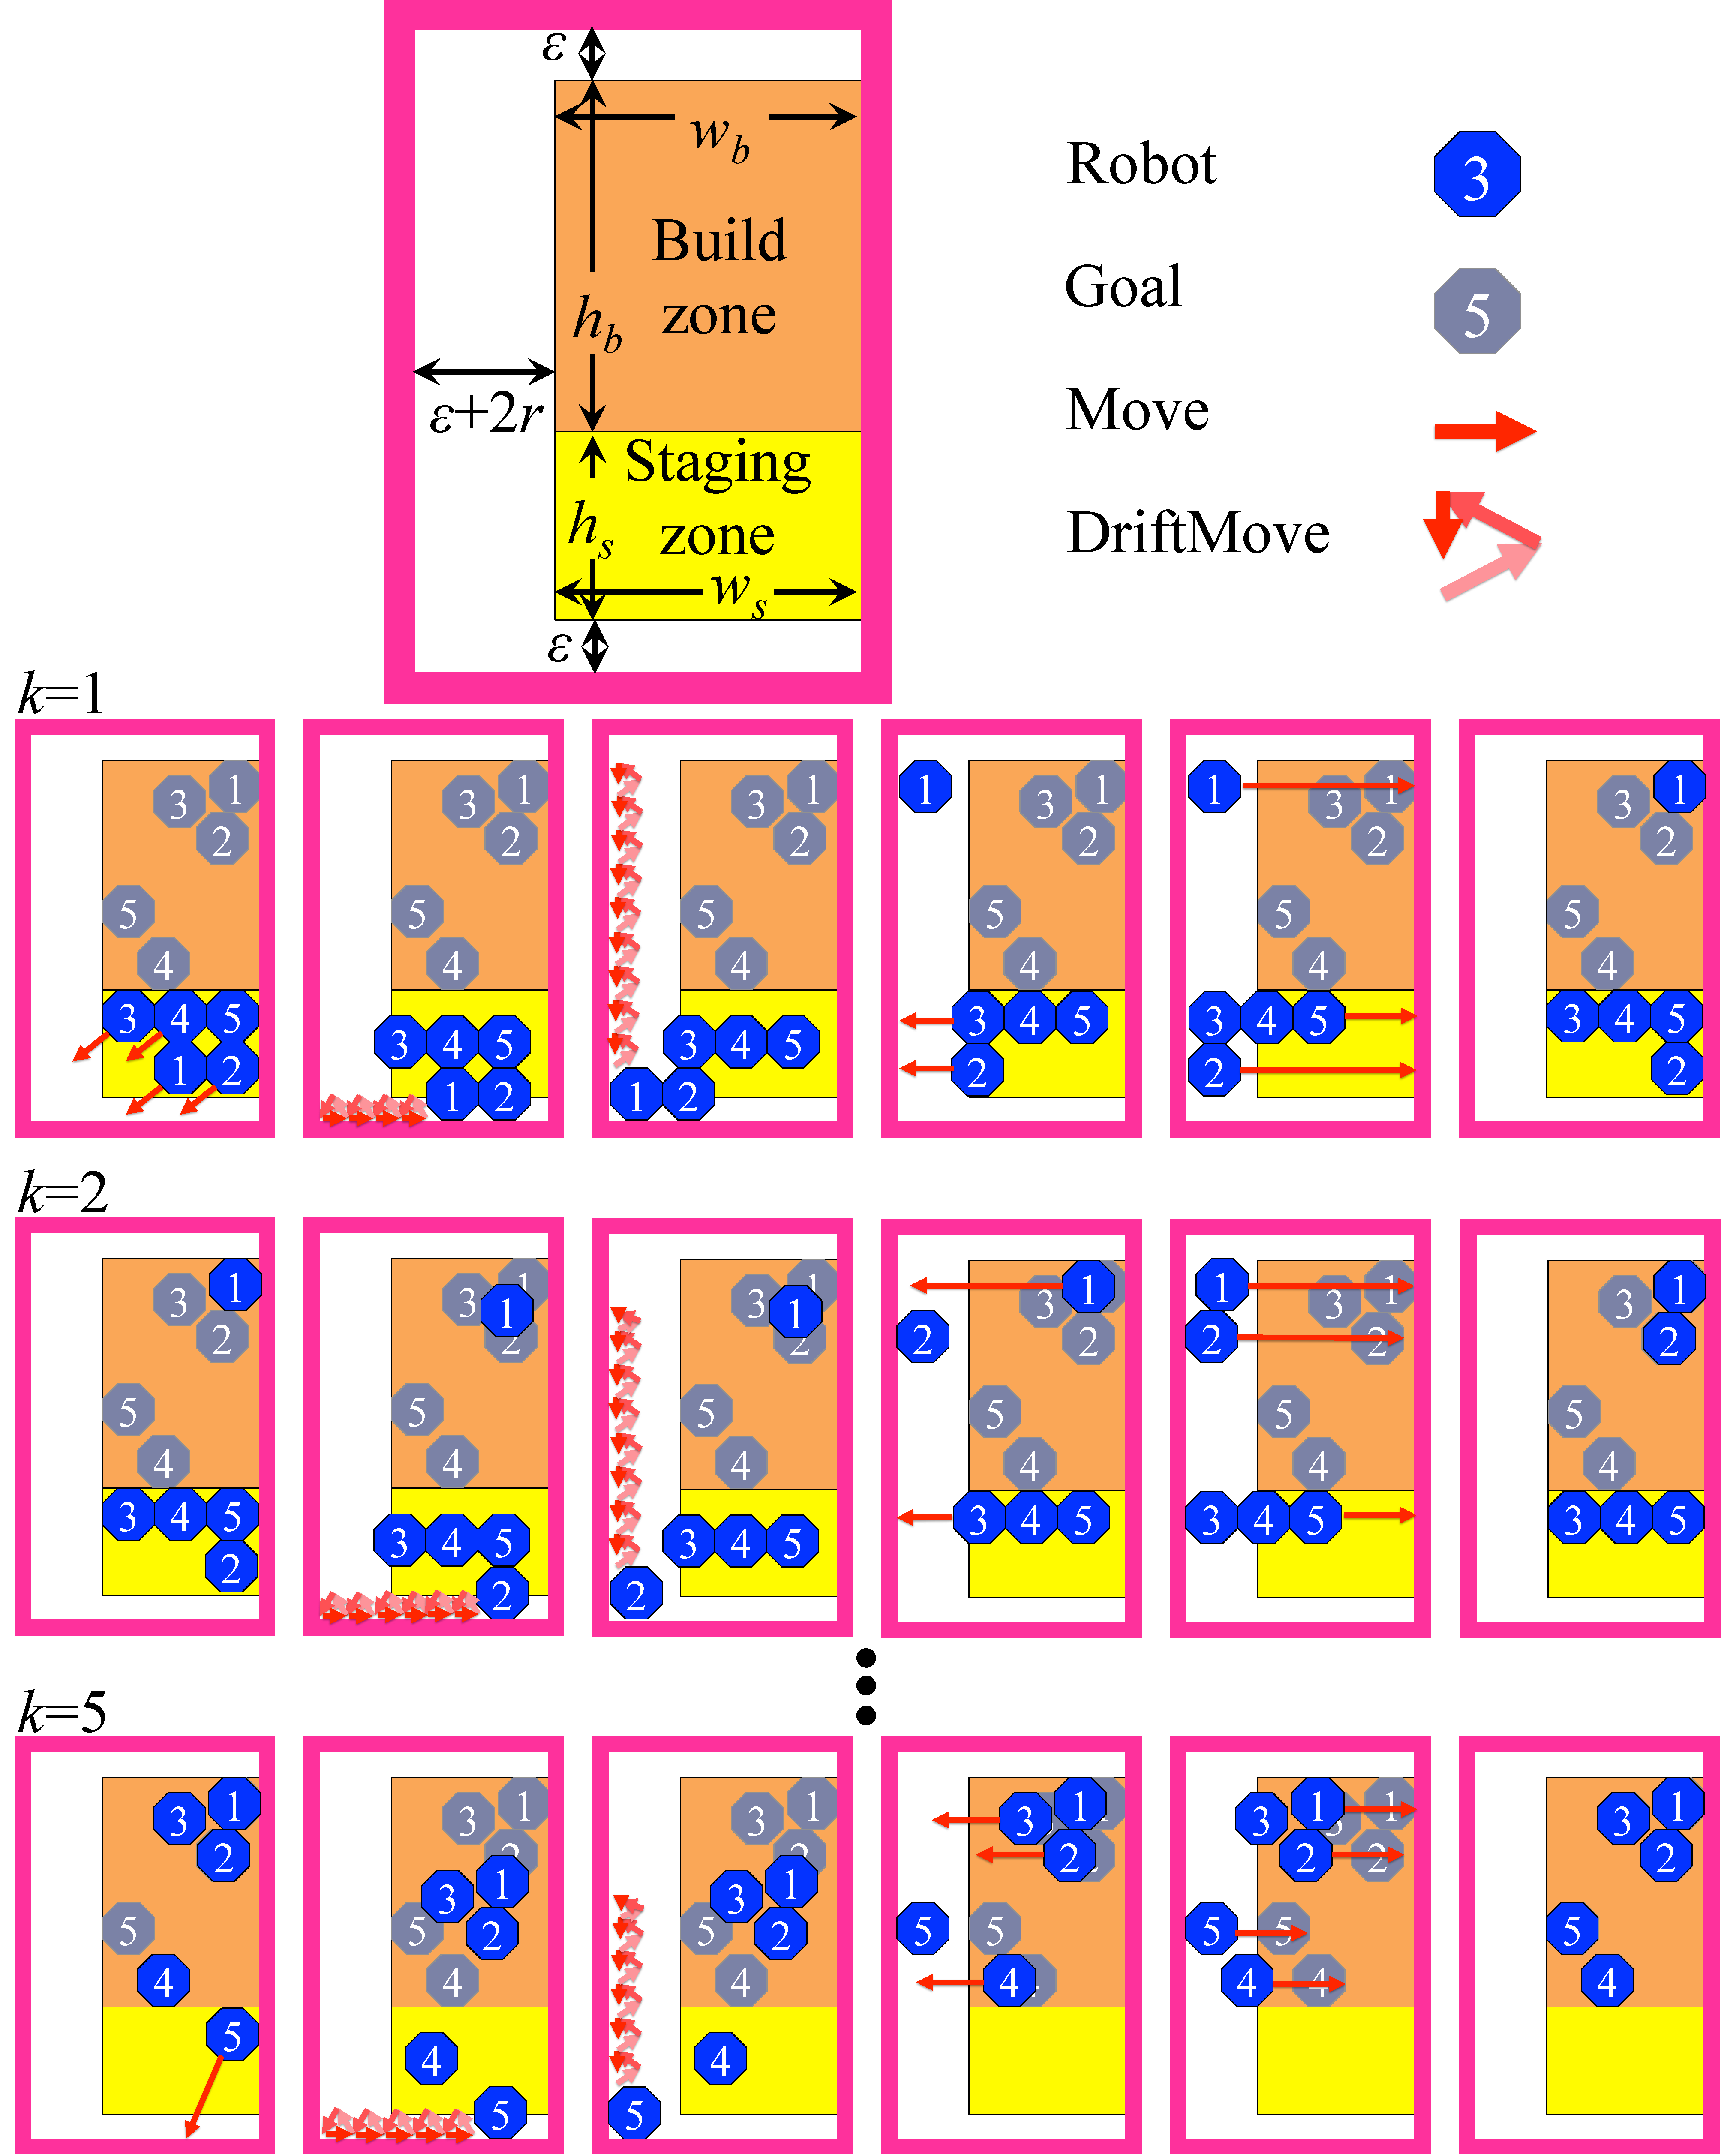
\includegraphics[width=1.0\columnwidth]{PositionNrobotsComp.pdf}
\end{center}
\vspace{-1em}
\caption{\label{fig:PositionNrobotsCont}
Illustration of Alg.\ \ref{alg:PosControlNRobots}, $n$ robot position control  using wall friction.
}
\end{figure}




\subsection{AutomaticCovControl.mp4}
A closed-loop controller that steers a swarm of particles to a desired covariance,  implemented with a box2D simulator. In this video the green ellipse is the desired covariance ellipse, the red ellipse is the current covariance ellipse of the swarm and the red dot is the mean position of the robots. Robots follow the algorithm to achieve the desired values for $\sigma_{goalxy}$, $\sigma_x^2$ and $\sigma_y^2$.

%%%%%%%%%%%%%%%%%%%%%%%%%%%%%
\section{ Algorithm for generating desired $y$ spacing between two robots using wall friction}\label{sec:2robotWallFriction}
\begin{algorithm}
\caption{GenerateDesired$y$-spacing($s_1,s_2,e_1,e_2,L$)}\label{alg:YControl}
\begin{algorithmic}[1]
\Require Knowledge of starting $(s_1,s_2)$ and ending $(e_1,e_2)$ positions of  two robots. 
$(0,0)$ is bottom corner, $s_1$ is rightmost robot, 
 $L$ is length of the walls. Current position of the robots are $(r_1,r_2)$.
\Ensure   $ r_{1x} - r_{2x}  \equiv s_{1x} - s_{2x} $   %$\Delta y(t) \equiv \Delta y(0)$ 
\State $ \Delta s_y  \gets s_{1y} - s_{2y} $
\State $ \Delta e_y \gets e_{1y} - e_{2y} $
\State $ r_1 \gets s_1$, $ r_2 \gets s_2$
\If {$\Delta e_y < 0 $ }
\State $ m \gets ( L-\max( r_{1y},r_{2y}) ,0)   $ \Comment{Move to top wall}
\Else 
\State  $ m \gets ( -\min( r_{1y},r_{2y}),0 )    $ \Comment{Move to bottom wall}
\EndIf
\State $m  \gets  m + (0, -\min( r_{1x},r_{2x} ))$ \Comment{Move to left}
\State $ r_1 \gets r_1+m$, $ r_2 \gets r_2+m$ \Comment{Apply move}
\If {$\Delta e_y - (r_{1y} - r_{2y} ) > 0 $}
\State $ m \gets (\min(|\Delta e_y - \Delta s_y |, L- r_{1y}), 0)$  \Comment{Move top}
\Else
\State $ m \gets (-\min(|\Delta e_y - \Delta s_y |, r_{1y}), 0)$\Comment{Move bottom}
\EndIf 
\State $m  \gets  m + (0, \epsilon)$ \Comment{Move right}
\State $ r_1 \gets r_1+m$, $ r_2 \gets r_2+m$ \Comment{Apply move}
\State $\Delta r_y = r_{1y} - r_{2y}$
\If {$\Delta r_y \equiv \Delta e_y$} 
\State   $ m \gets (e_{1x}-r_{1x}, e_{1y}-r_{1y})$
\State $ r_1 \gets r_1+m$, $ r_2 \gets r_2+m$ \Comment{Apply move}
\State  \Return $(r_1,r_2)$
\Else   
\State \Return GenerateDesired$y$-spacing($r_1,r_2,e_1,e_2,L$)
\EndIf
\end{algorithmic}
\end{algorithm}



%%%%%%%%%%%%%%%%%%%%%%%%%%%
\section{Calculations for modeling swarm as fluid in a simple planar workspace}\label{sec:fluidInPlanarRegion}
Two workspaces are used, a square and a circular workspace.

\subsection{Square Workspace}
This section provides formulas for the mean, variance,  covariance and correlation of a very large swarm of robots as they move inside a square workplace under the influence of gravity pointing in the direction $\beta$. The swarm is large, but the robots are small in comparison, and together cover an area of constant volume $A$. Under a global input such as gravity, they flow like water, moving to a side of the workplace and forming a polygonal shape. The workspace is 

The range of possible angles for the global input angle $\beta $ is [0,2$\pi $). In this range of angles, the swarm assumes eight different polygonal shapes. The shapes alternate between triangles and trapezoids when the area $A$$<$1/2, and alternate between squares with one corner removed and trapezoids when $A$$>$1/2.

Two representative formulas are attached, the outline of the swarm shapes in \eqref{tab:SquareRobotRegions} and $\bar{x}(\beta,A)$ in \eqref{tab:SquareXMean}.




\begin{figure}[h]
\begin{center}
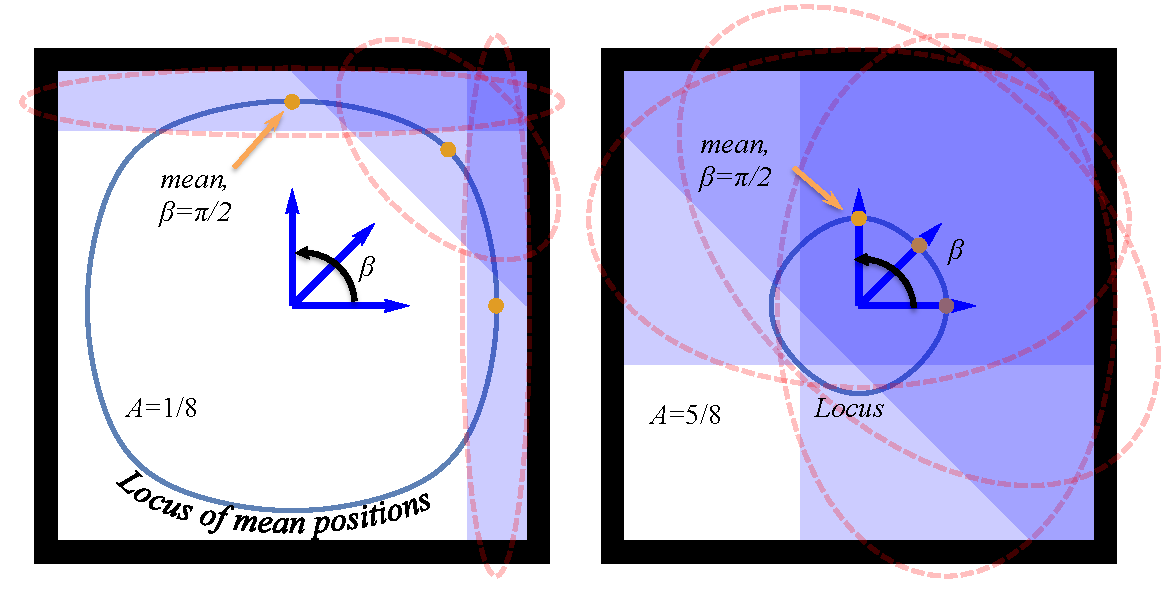
\includegraphics[width=\columnwidth]{SquarePlotPositions.pdf} 
\caption{A swarm in a square workspace under a constant global input assumes either a triangular or a trapezoidal shape if $A<1/2$.  If $A>1/2$ the swarm is either a squares with one corner removed or a trapezoidal  shape.}
\label{fig:friction}
\end{center}
\end{figure} 

\begin{table*}
\begin{align}
\bar{x}(\beta,A) = A\leq \frac{1}{2}: &\begin{cases}
 -\frac{\tan ^2(\beta )}{24 A}-\frac{A}{2}+1 & 0\leq \beta \leq \tan ^{-1}(2 A)\lor 2 \pi -\tan ^{-1}(2 A)<\beta \leq 2 \pi  \\
 1-\frac{1}{3} \sqrt{2} \sqrt{A \tan (\beta )} & \tan ^{-1}(2 A)<\beta \leq \frac{\pi }{2}-\tan ^{-1}(2 A) \\
 \frac{\cot (\beta )}{12 A}+\frac{1}{2} & \frac{\pi }{2}-\tan ^{-1}(2 A)<\beta \leq \tan ^{-1}(2 A)+\frac{\pi }{2} \\
 \frac{1}{3} \sqrt{2} \sqrt{-A \tan (\beta )} & \tan ^{-1}(2 A)+\frac{\pi }{2}<\beta \leq \pi -\tan ^{-1}(2 A) \\
 \frac{\tan ^2(\beta )}{24 A}+\frac{A}{2} & \pi -\tan ^{-1}(2 A)<\beta \leq \tan ^{-1}(2 A)+\pi  \\
 \frac{1}{3} \sqrt{2} \sqrt{A \tan (\beta )} & \tan ^{-1}(2 A)+\pi <\beta \leq \frac{3 \pi }{2}-\tan ^{-1}(2 A) \\
 \frac{1}{2}-\frac{\cot (\beta )}{12 A} & \frac{3 \pi }{2}-\tan ^{-1}(2 A)<\beta \leq \tan ^{-1}(2 A)+\frac{3 \pi }{2} \\
 1-\frac{1}{3} \sqrt{2} \sqrt{-A \tan (\beta )} & \tan ^{-1}(2 A)+\frac{3 \pi }{2}<\beta \leq 2 \pi -\tan ^{-1}(2 A) \\
\end{cases} \nonumber\\
\frac{1}{2}<A<1:&\begin{cases}
 -\frac{\tan ^2(\beta )}{24 A}-\frac{A}{2}+1 & 0\leq \beta \leq \tan ^{-1}\left(\frac{1}{2},1-A\right)\lor 2 \pi -\tan ^{-1}\left(\frac{1}{2},1-A\right)<\beta \leq 2 \pi  \\
 \frac{2 \sqrt{2} \sqrt{(1-A) \tan (\beta )} (A-1)+3}{6 A} & \tan ^{-1}\left(\frac{1}{2},1-A\right)<\beta \leq \frac{\pi }{2}-\tan ^{-1}\left(\frac{1}{2},1-A\right) \\
 \frac{6 A+\cot (\beta )}{12 A} & \frac{\pi }{2}-\tan ^{-1}\left(\frac{1}{2},1-A\right)<\beta \leq \tan ^{-1}\left(\frac{1}{2},1-A\right)+\frac{\pi }{2} \\
 \frac{-2 \sqrt{2} \sqrt{(A-1) \tan (\beta )} (A-1)+6 A-3}{6 A} & \tan ^{-1}\left(\frac{1}{2},1-A\right)+\frac{\pi }{2}<\beta \leq \pi -\tan ^{-1}\left(\frac{1}{2},1-A\right) \\
 \frac{\tan ^2(\beta )}{24 A}+\frac{A}{2} & \pi -\tan ^{-1}\left(\frac{1}{2},1-A\right)<\beta \leq \tan ^{-1}\left(\frac{1}{2},1-A\right)+\pi  \\
 \frac{2 \sqrt{2} \sqrt{(1-A) \tan (\beta )} (1-A)+6 A-3}{6 A} & \tan ^{-1}\left(\frac{1}{2},1-A\right)+\pi <\beta \leq \frac{3 \pi }{2}-\tan ^{-1}\left(\frac{1}{2},1-A\right) \\
 \frac{1}{2}-\frac{\cot (\beta )}{12 A} & \frac{3 \pi }{2}-\tan ^{-1}\left(\frac{1}{2},1-A\right)<\beta \leq \tan ^{-1}\left(\frac{1}{2},1-A\right)+\frac{3 \pi }{2} \\
 \frac{2 \sqrt{2} \sqrt{(A-1) \tan (\beta )} (A-1)+3}{6 A} & \tan ^{-1}\left(\frac{1}{2},1-A\right)+\frac{3 \pi }{2}<\beta \leq 2 \pi -\tan ^{-1}\left(\frac{1}{2},1-A\right) \\
\end{cases}
 \nonumber \\
A=1: &\frac{1}{2}
\end{align}
\protect\caption{$\bar{x}$ in a unit-square workspace}
\label{tab:SquareXMean}
\end{table*}



\begin{table*}
\tiny
\begin{align}
\text{RobotRegion}(\beta,A)= \nonumber 
A\leq \frac{1}{2}:&
\begin{cases}
 \left(
\begin{array}{cc}
 1 & 0 \\
 1 & 1 \\
 -A-\frac{\tan (\beta )}{2}+1 & 1 \\
 -A+\frac{\tan (\beta )}{2}+1 & 0 \\
\end{array}
\right) & 0\leq \beta \leq \tan ^{-1}(2 A)\lor 2 \pi -\tan ^{-1}(2 A)<\beta \leq 2 \pi  \\
 \left(
\begin{array}{cc}
 1 & 1 \\
 1-\sqrt{2} \sqrt{A \tan (\beta )} & 1 \\
 1 & 1-\sqrt{2} \sqrt{A \cot (\beta )} \\
\end{array}
\right) & \tan ^{-1}(2 A)<\beta \leq \frac{\pi }{2}-\tan ^{-1}(2 A) \\
 \left(
\begin{array}{cc}
 1 & 1 \\
 0 & 1 \\
 0 & -A+\frac{\cot (\beta )}{2}+1 \\
 1 & -A-\frac{\cot (\beta )}{2}+1 \\
\end{array}
\right) & \frac{\pi }{2}-\tan ^{-1}(2 A)<\beta \leq \tan ^{-1}(2 A)+\frac{\pi }{2} \\
 \left(
\begin{array}{cc}
 0 & 1 \\
 \sqrt{2} \sqrt{-A \tan (\beta )} & 1 \\
 0 & 1-\sqrt{2} \sqrt{-A \cot (\beta )} \\
\end{array}
\right) & \tan ^{-1}(2 A)+\frac{\pi }{2}<\beta \leq \pi -\tan ^{-1}(2 A) \\
 \left(
\begin{array}{cc}
 0 & 0 \\
 0 & 1 \\
 A-\frac{\tan (\beta )}{2} & 1 \\
 A+\frac{\tan (\beta )}{2} & 0 \\
\end{array}
\right) & \pi -\tan ^{-1}(2 A)<\beta \leq \tan ^{-1}(2 A)+\pi  \\
 \left(
\begin{array}{cc}
 0 & 0 \\
 0 & \sqrt{2} \sqrt{A \cot (\beta )} \\
 \sqrt{2} \sqrt{A \tan (\beta )} & 0 \\
\end{array}
\right) & \tan ^{-1}(2 A)+\pi <\beta \leq \frac{3 \pi }{2}-\tan ^{-1}(2 A) \\
 \left(
\begin{array}{cc}
 0 & 0 \\
 1 & 0 \\
 1 & A-\frac{\cot (\beta )}{2} \\
 0 & A+\frac{\cot (\beta )}{2} \\
\end{array}
\right) & \frac{3 \pi }{2}-\tan ^{-1}(2 A)<\beta \leq \tan ^{-1}(2 A)+\frac{3 \pi }{2} \\
 \left(
\begin{array}{cc}
 1 & 0 \\
 1-\sqrt{2} \sqrt{-A \tan (\beta )} & 0 \\
 1 & \sqrt{2} \sqrt{-A \cot (\beta )} \\
\end{array}
\right) & \tan ^{-1}(2 A)+\frac{3 \pi }{2}<\beta \leq 2 \pi -\tan ^{-1}(2 A) \\
\end{cases}
 %%%%%%%%%%%%%%%%%%%%%%%%%%%%%%%%%%
\nonumber \\
\frac{1}{2}<A<1:&
\begin{cases}
 \left(
\begin{array}{cc}
 1 & 0 \\
 1 & 1 \\
 (1-A)-\frac{\tan (\beta )}{2} & 1 \\
 (1-A)+\frac{\tan (\beta )}{2} & 0 \\
\end{array}
\right) & 0\leq \beta \leq \tan ^{-1}\left(\frac{1}{2},1-A\right)\lor 2 \pi -\tan ^{-1}\left(\frac{1}{2},1-A\right)<\beta \leq 2 \pi  \\
 \left(
\begin{array}{cc}
 1 & 0 \\
 1 & 1 \\
 0 & 1 \\
 0 & \sqrt{2} \sqrt{(1-A) \cot (\beta )} \\
 \sqrt{2} \sqrt{(1-A) \tan (\beta )} & 0 \\
\end{array}
\right) & \tan ^{-1}\left(\frac{1}{2},1-A\right)<\beta \leq \frac{\pi }{2}-\tan ^{-1}\left(\frac{1}{2},1-A\right) \\
 \left(
\begin{array}{cc}
 0 & 1 \\
 1 & 1 \\
 1 & (1-A)-\frac{\cot (\beta )}{2} \\
 0 & (1-A)+\frac{\cot (\beta )}{2} \\
\end{array}
\right) & \frac{\pi }{2}-\tan ^{-1}\left(\frac{1}{2},1-A\right)<\beta \leq \tan ^{-1}\left(\frac{1}{2},1-A\right)+\frac{\pi }{2} \\
 \left(
\begin{array}{cc}
 1 & 1 \\
 0 & 1 \\
 0 & 0 \\
 1-\sqrt{2} \sqrt{-(1-A) \tan (\beta )} & 0 \\
 1 & \sqrt{2} \sqrt{-(1-A) \cot (\beta )} \\
\end{array}
\right) & \tan ^{-1}\left(\frac{1}{2},1-A\right)+\frac{\pi }{2}<\beta \leq \pi -\tan ^{-1}\left(\frac{1}{2},1-A\right) \\
 \left(
\begin{array}{cc}
 0 & 0 \\
 0 & 1 \\
 -(1-A)-\frac{\tan (\beta )}{2}+1 & 1 \\
 -(1-A)+\frac{\tan (\beta )}{2}+1 & 0 \\
\end{array}
\right) & \pi -\tan ^{-1}\left(\frac{1}{2},1-A\right)<\beta \leq \tan ^{-1}\left(\frac{1}{2},1-A\right)+\pi  \\
 \left(
\begin{array}{cc}
 1 & 0 \\
 0 & 0 \\
 0 & 1 \\
 1-\sqrt{2} \sqrt{(1-A) \tan (\beta )} & 1 \\
 1 & 1-\sqrt{2} \sqrt{(1-A) \cot (\beta )} \\
\end{array}
\right) & \tan ^{-1}\left(\frac{1}{2},1-A\right)+\pi <\beta \leq \frac{3 \pi }{2}-\tan ^{-1}\left(\frac{1}{2},1-A\right) \\
 \left(
\begin{array}{cc}
 1 & 0 \\
 0 & 0 \\
 0 & -(1-A)+\frac{\cot (\beta )}{2}+1 \\
 1 & -(1-A)-\frac{\cot (\beta )}{2}+1 \\
\end{array}
\right) & \frac{3 \pi }{2}-\tan ^{-1}\left(\frac{1}{2},1-A\right)<\beta \leq \tan ^{-1}\left(\frac{1}{2},1-A\right)+\frac{3 \pi }{2} \\
 \left(
\begin{array}{cc}
 0 & 0 \\
 1 & 0 \\
 1 & 1 \\
 \sqrt{2} \sqrt{-(1-A) \tan (\beta )} & 1 \\
 0 & 1-\sqrt{2} \sqrt{-(1-A) \cot (\beta )} \\
\end{array}
\right) & \tan ^{-1}\left(\frac{1}{2},1-A\right)+\frac{3 \pi }{2}<\beta \leq 2 \pi -\tan ^{-1}\left(\frac{1}{2},1-A\right) \\
\end{cases},\nonumber\\
%%%%%%%%%%%%%%%%%%%%%%%%%%%%%%%
A=1:&\left(
\begin{array}{cc}
 1 & 0 \\
 0 & 0 \\
 0 & 1 \\
 1 & 1 \\
\end{array}
\right)
\end{align}
\protect\caption{RobotRegions in a unit-square workspace}
\label{tab:SquareRobotRegions}
\end{table*}


\subsection{Circle Workspace}
The area under a chord of a circle is the area of a sector less the area of the triangle originating at the circle center: 
$A=S(sector)-S(triangle)=1/2 LR-1/2 C(1-h)$, thus
\begin{align}
A=(1/2)\left[LR-c(R-h)\right]
\end{align}
where $L$ is arc length, $c$ is chord length, $R$ is radius and $h$ is height. Solving for $L$ and $C$ gives
\begin{align}
L&=2 \cos ^{-1}(1-h)\\
C&=2\sqrt{h(2-h)}
\end{align}
Therefore the area under a chord is
\begin{align}
\cos ^{-1}(1-h)-(1-h) \sqrt{(2-h) h}
\end{align}

For a circular workspace, with $\beta = 0$, the variance of $x$ and $y$ are:
{\tiny
\begin{align}
&\sigma_x^2(h)=\frac{64 (h-2)^3 h^3}{144 \left(\sqrt{-(h-2) h} (h-1)+\arccos(1-h)\right)^2} +\nonumber\\
&\frac{9 \left(\sqrt{-(h-2) h} (h-1)+\arccos(1-h)\right) \left(\sin \left(4 \arcsin(1-h)\right)+4 \arccos(1-h)\right)}{144 \left(\sqrt{-(h-2) h} (h-1)+\arccos(1-h)\right)^2}
\end{align}}

{\tiny
\begin{align}
\sigma_y^2(h)=
\frac{12 \arccos(1-h)-8 \sin \left(2 \arccos(1-h)\right)+\sin \left(4 \arccos(1-h)\right)}{48 \left(\sqrt{-(h-2) h} (h-1)+\arccos(1-h)\right)}
\end{align}}

For $\beta = 0$, $\sigma_{xy}=0$. These values can be rotated to calculate $\sigma_x^2(\beta,h),\sigma_y^2(\beta,h),$ and $\sigma_{xy}(\beta,h)$.

%%%%%%%%%%%%%%%%%%%%%%%%%%%%%%
\section*{Acknowledgments}
This work was supported by the National Science Foundation under Grant No.\ \href{http://nsf.gov/awardsearch/showAward?AWD_ID=1553063}{ [IIS-1553063]}.

%%%%%%%%%%%%%%%
%% Use plainnat to work nicely with natbib. 
\bibliographystyle{plainnat}
\footnotesize
\bibliography{IEEEabrv,ShapingSwarmFrictionSharedInput}
%\end{document}



